In the last chapter, we have covered means to understand variability,
synthesize variability models for a given software system, and to select sample
sets of configurations. To enable the assessment of performance evolution for
configurable software systems, the next step in our methodology takes into
account the dimension of diachrony. As software evolves, multiple versions, or
called revisions, of a software system exist. In this chapter, we address the
question of how we can assess performance for multiple revisions. Moreover, we
ask whether we can describe a configurable software systems’ performance
evolution without exhaustively assessing all versions by selecting only a
sample set of versions. As illustrated in the methodological road-map in
Figure~\ref{fig:roadmap_2}, we summarize these two questions with the task of
revision sampling.

\begin{figure}[h!]
	\centering
	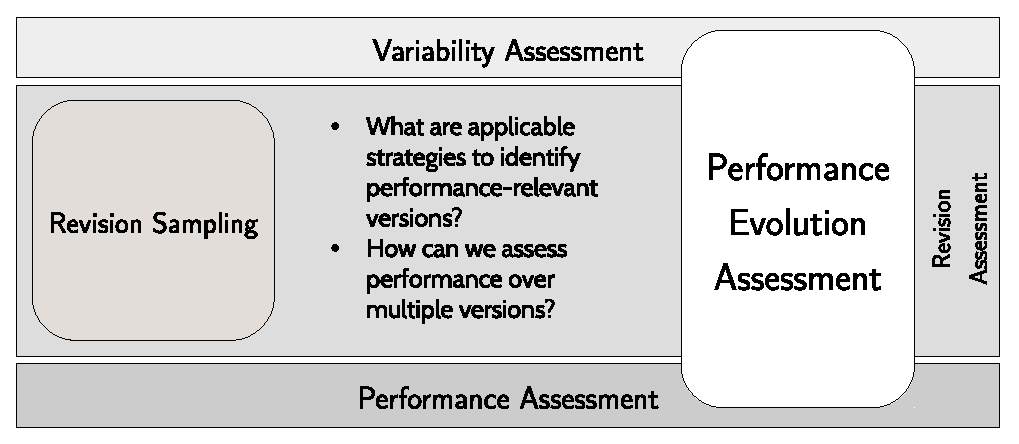
\includegraphics[width=0.75\textwidth]{images/process_revassesment.eps}
	\caption{Methodological road-map: questions to address with revision
	assessment.}
	\label{fig:roadmap_2}
\end{figure}

The chapter is organized as follows. In section~\ref{sec:towards_revsampling} we
present the methodological requirements for a designing and selecting a revision sampling
strategy. In section ~\ref{sec:revsampling_strat} we propose five approaches to
revision sampling based on observations of configurable software systems. In
section~\ref{sec:revsampling_eval} we evaluate the different approaches against
exhaustive measurements of a selection of configurable software systems.
Finally, in section~\ref{sec:revsampling_method} we conclude the chapter and
discuss the approaches' applicability in the context of our methodology.

\section{Towards Revision Sampling}\label{sec:towards_revsampling}
Research so far has addressed the assessment of a software system’s revision
history under the umbrella of repository mining, for instance, to localize bugs
\citep{moin_bug_2010} or performance regression \citep{heger_automated_2013}.
Nonetheless, so far there exists little to no research addressing the question
what the choice of versions might reveal about performance evolution. The task
of selecting resources and a sample set of versions to analyze can be conceived
as a sampling strategy, where the objective is to cover interesting entities
(performance changes, in our case) while trying to limit the sample size to
keep the required effort reasonable. Before we present different approaches to
select a sample set of revisions, we need to define general cornerstones for
evaluating a sample set of revisions as well as respective revision sampling
strategies with respect to performance change history.

\paragraph{Revision Sample Set.} The first question is, what criteria we take as
a basis for rating a sample set of revisions as \emph{meaningful}. First, our intention
is to obtain a representative description of a software system’s performance
change history while only assessing a fraction of revisions. That is, assessing
a representative sample of revisions should yield a performance change history
similar to the assessment of all revisions. Since we are interested in
revisions for which performance measurements change, these revisions should be
contained in a representative sample. Second, especially in the context of
variability, a performance change might only affect a subset of the assessed
configurations. A representative sample set, therefore, should describe a
history of significant performance changes with respect to all variants
assessed. We consider a performance change to be significant, if it affects a
significant portion of the sample of variants (effect range) and if the
relative change in performance measurements is significantly huge (effect
magnitude).

\begin{figure}[h!]
	\centering
	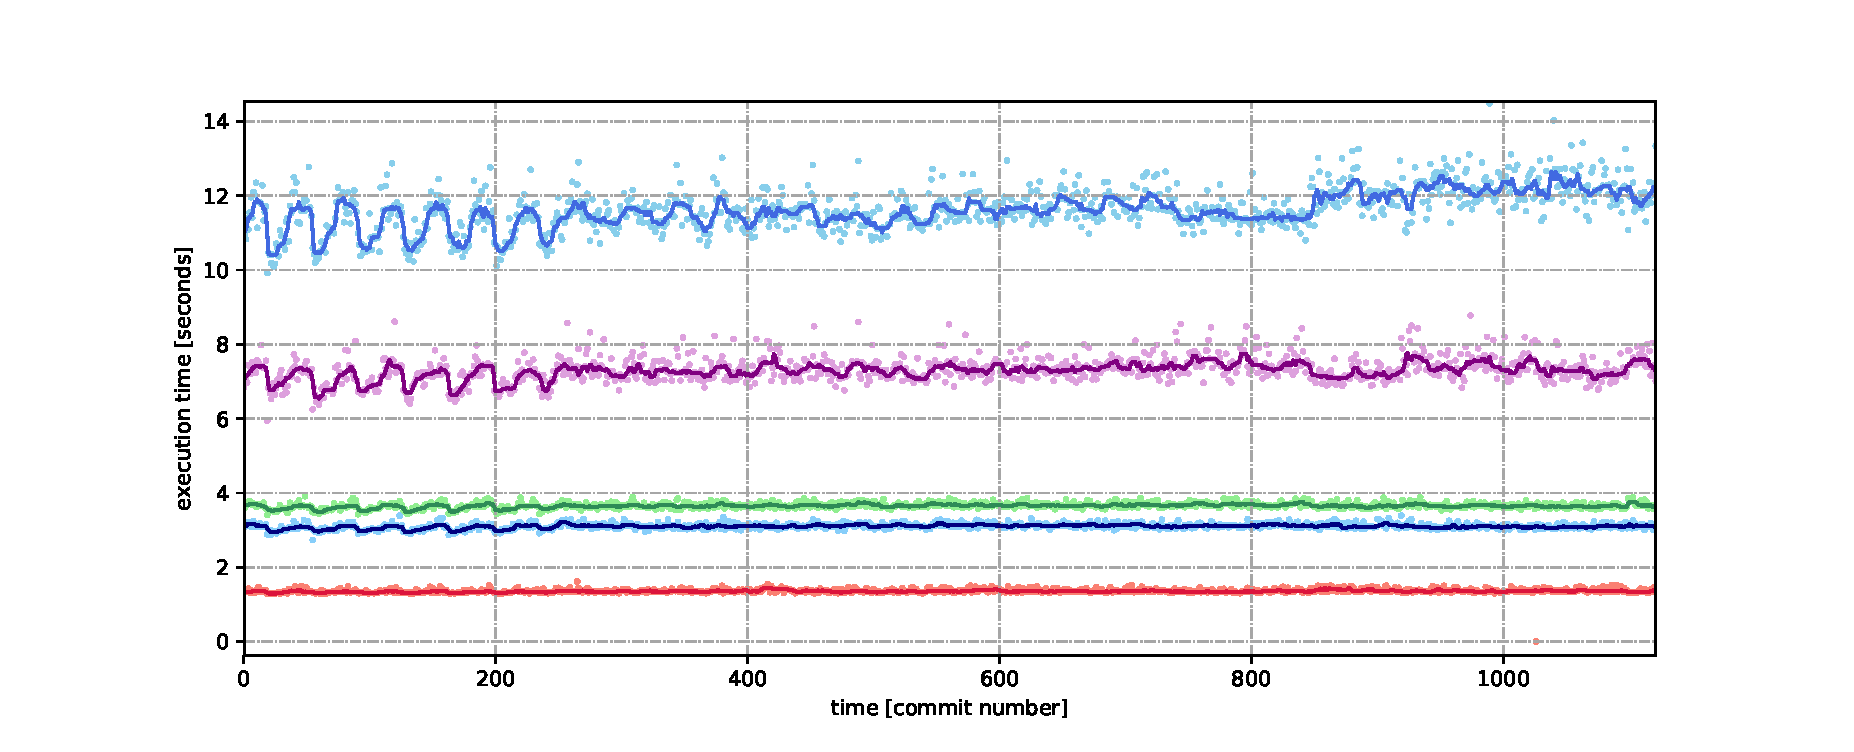
\includegraphics[width=0.95\textwidth]{images/xz_sample_evolution.eps}
	\caption{Performance History for XZ}
	\label{fig:xz_evosample}
\end{figure}

To illustrate the two facets of performance changes, in
Figure~\ref{fig:xz_evosample} we see a history of performance measurements (execution time in this case) for a
small-scale configurable software system, file compression tool called \emph{GNU
XZ Utils}. The graphic depicts execution time measures for executing a standard
compression benchmark for $1,135$ different versions and covers a version
history of about nine years. In this excerpt, we only show the execution time measures
of four different variants, i.e., each version was assessed with four different
configurations. One can see that the execution time for the red and the green
configurations remains stable and does not fluctuate, while for the blue and
grey configuration, the execution time measures are generally more volatile.
Moreover, between 2010 and 2012, performance for the latter variants fluctuates
heavily. With regard to the two facets of significance mentioned above, not all
variants are affected similarly by this effect. That is, if performance were
assessed solely for one of the non-fluctuating variants, no performance
evolution could be identified.

While the former significance criterion can unambiguously defined by a threshold
number of variants, for the latter one one needs to define how to summarize
relative performance change among all variants. For instance, a performance
change may have a significant magnitude, if the average deviation of
performance measurements for all variants is greater than a specified threshold
value.

\paragraph{Revision Sampling Strategies.} The second question addresses the
rationale behind a revision sampling strategy. To obtain representative sample sets, sampling
strategies are intended to utilize knowledge about the total volume to select
sample sets from. For instance, pair-wise sampling aims to cover most feature
interactions. Similarly, we demand for a meaningful revision sampling strategy
to exhibit a certain rationale or coverage criterion. If we conceive a sampling
strategy as a binary classificator that, in our case, decides whether in a
revision a performance change is likely, or performance measurements might have
changed compared to prior commits, we want  this classifier to be sensitive,
i.e., to have a preferably high true positive rate. That is, a sampling
strategy is meaningful if we learn which revision features most likely indicate
performance evolution.
 
\section{Revision Sampling Strategies}\label{sec:revsampling_strat}

\begin{figure}[h!]
\centering
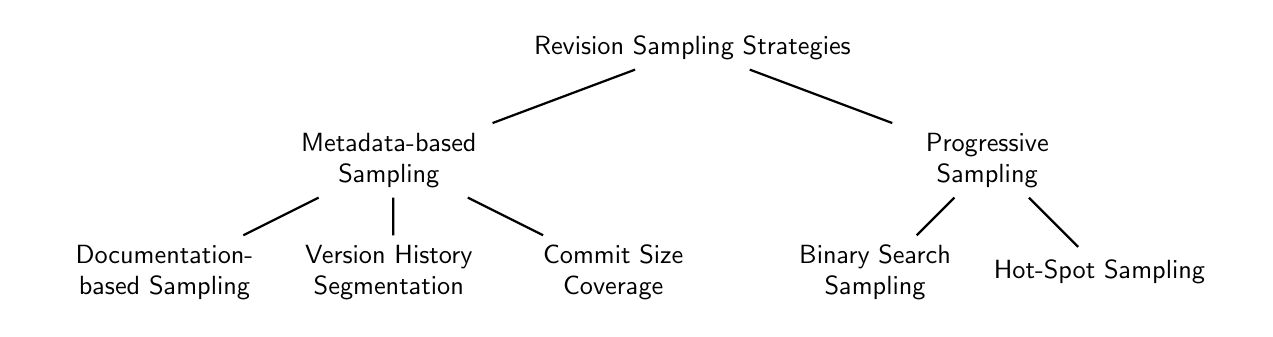
\begin{tikzpicture}[%sibling distance=15em,
level 1/.style={sibling distance=8cm},
level 2/.style={sibling distance=3cm}, 
level 3/.style={sibling distance=6cm},
  every node/.style = {rounded corners,
    draw, align=center,
    top color=white, bottom color=blue!20},thick,scale=0.95, every
    node/.style={scale=0.95}]
  \node {\sffamily Revision Sampling Strategies}
    child { 
    	node [align=left] {
    		\begin{tabular}{c} 
    			{\sffamily \parbox{3cm}{\centering Metadata-based Sampling}}
    		\end{tabular}
    	}
    	child { 
    		node [align=left] {
    			\begin{tabular}{c}
    				{\sffamily \parbox{3cm}{\centering Documentation-based Sampling}}
    			\end{tabular}
    		}
    	} 
    	child { 
    		node [align=left] {
    			\begin{tabular}{c} 
    				{\sffamily \parbox{3cm}{\centering Version History Segmentation}}
    			\end{tabular}
    		}
    	}
    	child { 
    		node [align=left] {
    			\begin{tabular}{c} 
    				{\sffamily \parbox{3cm}{\centering Commit Size Coverage}}
    			\end{tabular}
    		}
    	} 
    }
    child { 
    	node [align=left] {
    		\begin{tabular}{c} 
    			{\sffamily \parbox{3cm}{\centering Progressive Sampling}}
    		\end{tabular}
    	} 
    	child { 
    		node [align=left] {
    			\begin{tabular}{c}
    				{\sffamily \parbox{3cm}{\centering Binary Search Sampling}}
    			\end{tabular}
    		}
    	} 
    	child { 
    		node [align=left] {
	    		\begin{tabular}{c} 
	    			{\sffamily \parbox{3cm}{\centering Hot-Spot Sampling}}
	    		\end{tabular}
    		}
    	} 
    };
\end{tikzpicture}
\caption{Overview of our proposed revision
sampling strategies.}\label{fig:revsampling_overview}
\end{figure}

\subsection{Documentation-driven Sampling}
\subsection{Version History Segmentation}
\subsection{Change Coverage Sampling}
\subsection{Binary-Search-based Sampling}
\subsection{Hot-Spot Sampling}

\section{Strategy Evaluation}\label{sec:revsampling_eval}
\section{Methodological Remarks}\label{sec:revsampling_method}

%\begin{figure}
%\def\tabularxcolumn#1{m{#1}}
%\begin{tabularx}{\linewidth}{@{}cXX@{}}
%\begin{tabular}{c}
%\subfloat[Activity Graph for \texttt{GNU XZ}, generated from 399 versions
%between March 24, 2017, and August 14, 2017. The earliest release version is
%\texttt{5.1.1alpha}, the latest is \texttt{5.3.0alpha}.]
%{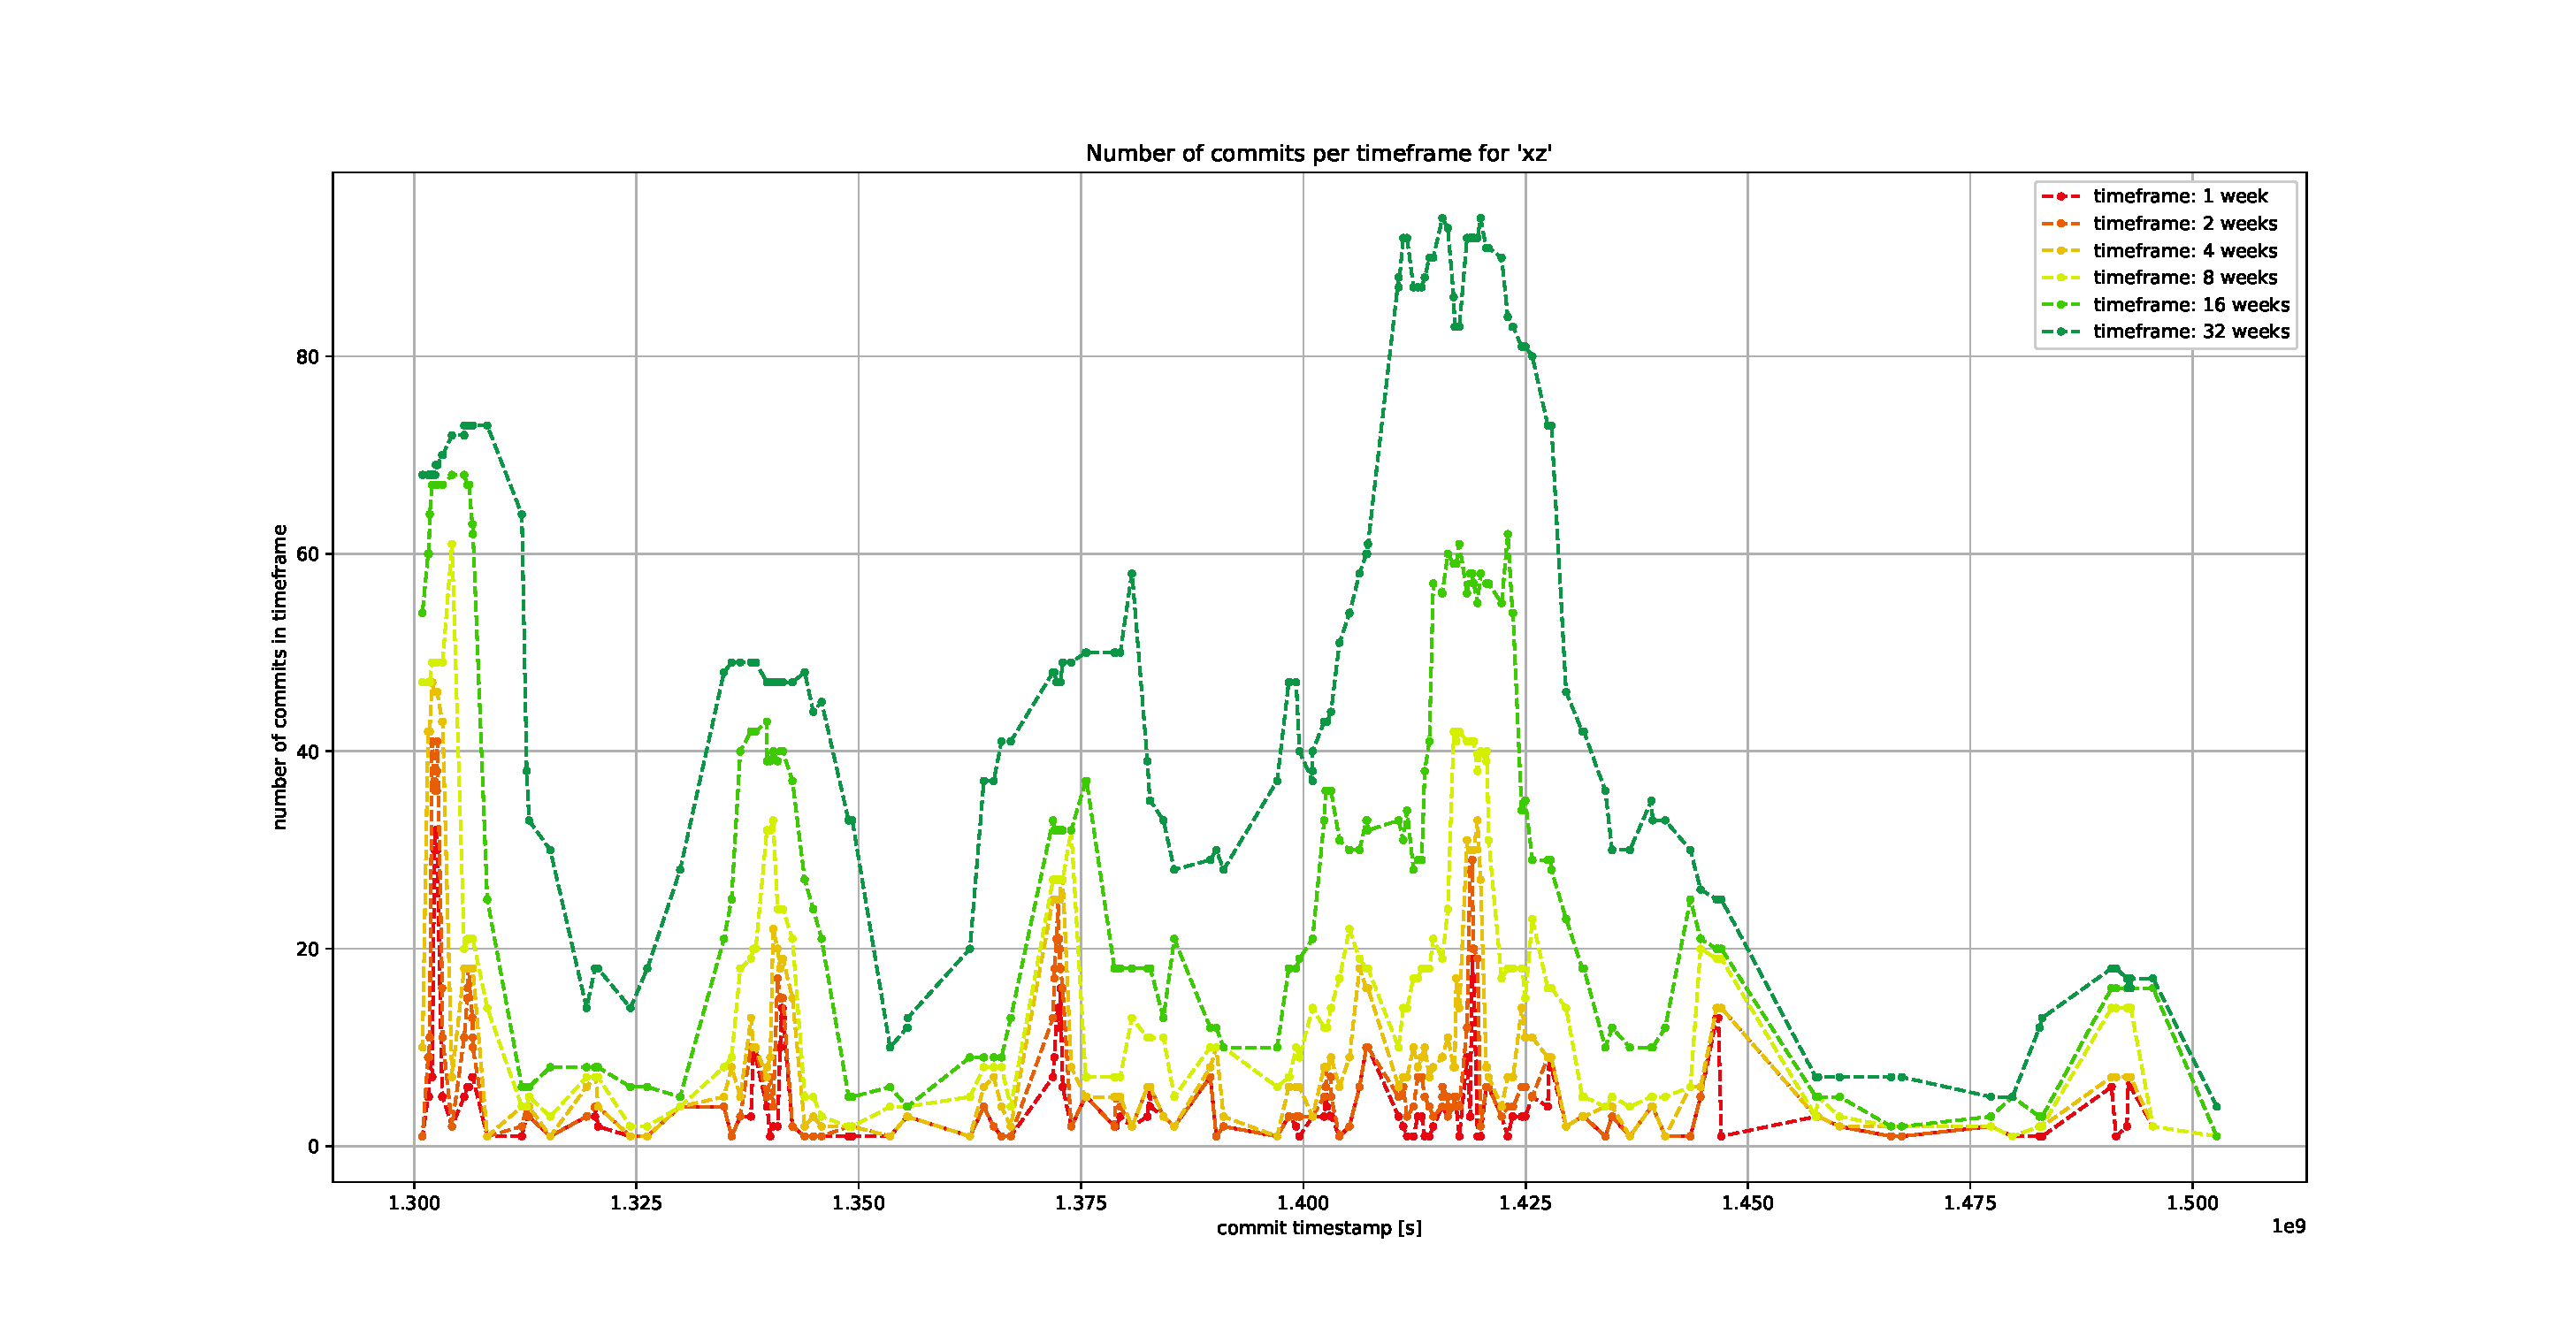
\includegraphics[width=0.99\textwidth]{images/activity_xz.eps}}
%\\
%\subfloat[Activity Graph for \texttt{x264}, generated from 2851 versions
%between June 3, 2004, and June 26, 2017. The earliest release version is
%\texttt{BUILD 1} from, the latest is \texttt{BUILD 149} from
%X.]{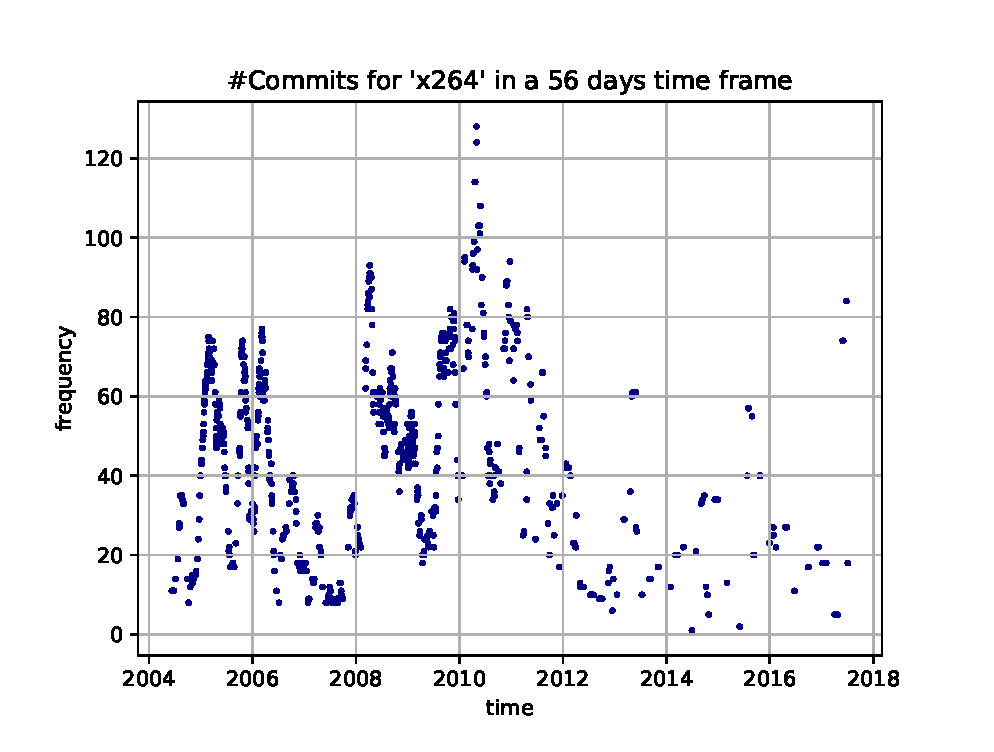
\includegraphics[width=0.99\textwidth]{images/activity_x264.eps}}\\
%\end{tabular}
%\end{tabularx}
%\caption{Commit activity for two sample systems, the compression
%utility \texttt{GNU XZ} and the video encoder \texttt{x264}. For each version,
%the activity is measured as the number of commits that were pushed within a
%certain timeframe after or before the actual commit. The timeframes range from
%one week to 32 weeks, as shown in the legendary.}
%\label{fig:ActivityGraphs}
%\end{figure}
